\documentclass[12pt,a4paper]{report}
\usepackage[top=0.70in, bottom=0.70in, left=0.8in,right=0.80in]{geometry}
\usepackage[pdftex]{graphicx}
\usepackage[bookmarks,colorlinks=false]{hyperref}
\hypersetup{pdfborder = {0 0 0}}
\usepackage{verbatim}
\usepackage[final]{pdfpages} 
\usepackage{float}
\usepackage{hyperref}
\usepackage{pslatex}
\usepackage{array}
\usepackage{setspace}
\usepackage{float}
\usepackage[autostyle=false, style=english]{csquotes}
\MakeOuterQuote{"}
\usepackage{enumerate}
\usepackage{longtable}
\usepackage{listingsutf8}
\usepackage{color}
\definecolor{codegreen}{rgb}{0,0.6,0}
\definecolor{codegray}{rgb}{0.5,0.5,0.5}
\definecolor{codepurple}{rgb}{0.58,0,0.82}
\definecolor{backcolour}{rgb}{0.95,0.95,0.92}

\lstdefinestyle{mystyle}{
	backgroundcolor=\color{backcolour},   
	commentstyle=\color{codegreen},
	keywordstyle=\color{magenta},
	numberstyle=\tiny\color{codegray},
	stringstyle=\color{codepurple},
	basicstyle=\footnotesize,
	breakatwhitespace=false,         
	breaklines=true,                 
	captionpos=b,                    
	keepspaces=true,                 
	numbers=left,                    
	numbersep=5pt,                  
	showspaces=false,                
	showstringspaces=false,
	showtabs=false,                  
	tabsize=2
}

\lstset{
	style=mystyle,
	inputencoding=utf8/latin1
}

\usepackage[font=small,labelfont=bf]{caption}
\def\figurename{\textbf{Figure }}
\usepackage{fancyhdr}
\fancypagestyle{plain}
{
    \fancyfoot[L]{\emph{Administraci\'on de Servicios en Red}}
    \fancyfoot[R]{\thepage}
    \renewcommand{\headrulewidth}{0.4pt}
    \renewcommand{\footrulewidth}{0.4pt}
}
\pagestyle{fancy}
\rhead{\emph{Pr\'actica 3}}
\fancyfoot[LO,LE]{\emph{Administraci\'on de Servicios en Red}}
\cfoot{}
\fancyfoot[RO, RE]{\thepage}
\renewcommand{\headrulewidth}{0.4pt}
\renewcommand{\footrulewidth}{0.4pt}
\usepackage{pgf}
\usepackage{pgfpages}
\pgfpagesdeclarelayout{boxed}
{ \edef\pgfpageoptionborder{0pt}}
{ 
    \pgfpagesphysicalpageoptions {logical pages=0,} 
    \pgfpageslogicalpageoptions{1}
    {
        border code=\pgfsetlinewidth{2pt}\pgfstroke,%
        border shrink=\pgfpageoptionborder,%
        resized width=.95\pgfphysicalwidth,%
        resized height=.95\pgfphysicalheight,%
        center=\pgfpoint{.5\pgfphysicalwidth}{.5\pgfphysicalheight}%
    }
}
\pgfpagesuselayout{boxed}
\setlength{\parindent}{1cm}
\usepackage[utf8]{inputenc}
\usepackage[spanish]{babel} 
\begin{document}
\renewcommand\bibname{Referencias Bibliogr\'aficas}
\lhead{ }
%-------------PORTADA Y CONTRAPORTADA--------------%
\newpage
\begin{center}
\thispagestyle{empty}
\LARGE{\textsc {\textbf{INSTITUTO POLITÉCNICO NACIONAL}}}\\[0.5cm]
\Large{\textbf{ESCUELA SUPERIOR DE CÓMPUTO}}\\[0.7cm]
\vspace*{2cm}
\LARGE{\textbf{\\PRÁCTICA 3: MONITOREO DE SERVICIOS DE RED\\}}
\vspace*{1cm}
\Large{\textbf{ADMINISTRACIÓN DE SERVICIOS EN RED\\}}
\vspace*{2cm}
\end{center}
\large{\textbf{\\EQUIPO 1 (Evaluación 4), EQUIPO 4 (Evaluación 5):}}\\
\vspace*{.5cm}
\large{\textsc{\\+ HERNÁNDEZ PINEDA MIGUEL ANGEL}}\\
\large{\textsc{\\+ MONROY MARTOS ELIOTH}}\\
\large{\textsc{\\+ ORTA CISNEROS SABRINA}}\\
\large{\textsc{\\+ RAMÍREZ CENTENO HUGO ENRIQUE}}\\
\large{\textsc{\\+ SALDAÑA AGUILAR ANDRÉS ARNULFO}}\\
\large{\textsc{\\+ ZÚÑIGA HERNÁNDEZ CARLOS}}\\
\vspace*{0.5cm}
\large{\textbf{\\PROFRA. TANIBET PÉREZ DE LOS SANTOS MONDRAGÓN}}\\
\vspace*{0.5cm}
\begin{flushright}
\Large{\textbf{\\18 de Mayo 2019}}
\end{flushright}
\newpage
%-------------INDICE-------------------------------%
\pagenumbering{roman}
\pagestyle{empty}
\addtocontents{toc}{\protect\thispagestyle{empty}}
\tableofcontents
\addtocontents{lof}{\protect\thispagestyle{empty}}
%\listoffigures
\cleardoublepage
\pagestyle{fancy}
\newpage
\pagenumbering{arabic}
%---------------CONTENIDO-------------------------%
\newpage
\chapter{Descripción de la Prueba}
\section{Propósito de la prueba}
\noindent
El presente documento tiene como objetivo la ejecución de las pruebas sobre el Sistema de Administración Escolar (en adelante SAES) con base en la especificación técnica.
\section{Alcance}
\noindent
Las pruebas que se presentan a continuación son pruebas unitarias de cada uno de los casos de uso del SAES.
\begin{itemize}
    \item Inicios de sesión en los diferentes perfiles.
    \item Registro de usuarios.
    \item Registro de materias.
    \item Registro de profesores.
    \item Registro de grupos.
    \item Generación de citas de inscripción.
    \item Reinscripción del alumno.
    \item Creación y almacenamiento de horarios.
    \item Edición de registros.
    \item Etcétera
\end{itemize}
\section{Elementos involucrados}
\noindent
Como se mencionó anteriormente se trabajará con todos los Casos de Uso que conforman el sistema, por lo tanto se verificarán todas las pantallas, así como los mensajes de alerta, confirmación y error que muestra el sistema. Los mensajes así como las pantallas del sistema se pueden encontrar en la sección de Anexos.
\section{Requerimientos}
\noindent
Las pruebas se ejecutarán en el laboratorio de la Escuela Superior de Cómputo haciendo uso de los equipos que se encuentran ahí. Es necesario tener las computadoras conectadas a una red local y que cada una de ellas tenga conexión con un equipo que será designado como el servidor. El navegador a ocupar será \textit{Google Chrome}.
\begin{longtable}{ | p{8cm} | p{7cm} | }
\hline
\multicolumn{2}{|p{15cm}|}{\textbf{Datos de Prueba}}\\
\hline
\textbf{Tipo de Prueba}: & Completa\\
\hline
\textbf{Fecha de Aplicación}: & \\
\hline
\textbf{Hora Inicio}: & \\
\hline
\textbf{Hora Final}: & \\
\hline
\textbf{Nombre del líder de pruebas}: & \\
\hline
\textbf{Nombre del tester}: & \\
\hline
\end{longtable}
\section{Checklist}
\noindent
Para poder dar inicio con las pruebas compruebe que cuenta con los siguientes puntos: \begin{itemize}
    \item Lápiz.
    \item Guión de Pruebas.
    \item El equipo cuenta con conexión al servidor.
    \item El equipo cuenta con el navegador Google Chrome.
\end{itemize}
\section{Instrucciones}
\begin{itemize}
    \item Verifique que cuenta con conexión al servidor de pruebas.
    \item Abra el navegador Google Chrome.
    \item Ingrese la siguiente dirección: 
\end{itemize}
\chapter{Desarrollo y Resultados}
\section{Examen 1.- Administración de fallas con mínimos cuadrados}
\subsection{Ejercicio 1: Definición de umbrales}
\noindent
Para llevar a cabo la definición de umbrales, realizamos el método propuesto por CISCO; consiste en hacer una lectura de datos por un periodo de tiempo (en este caso fueron 10 minutos), almacenar los datos obtenidos y generar una tabla de dispersión y con base en ella definir el umbral GO (umbral mayor) y a partir de este definir los umbrales inferiores. En este caso el agente que íbamos a monitorear se nos fue proporcionado por la profesora, el cual tenía los siguientes valores.
\begin{figure}[H]
  \centering
    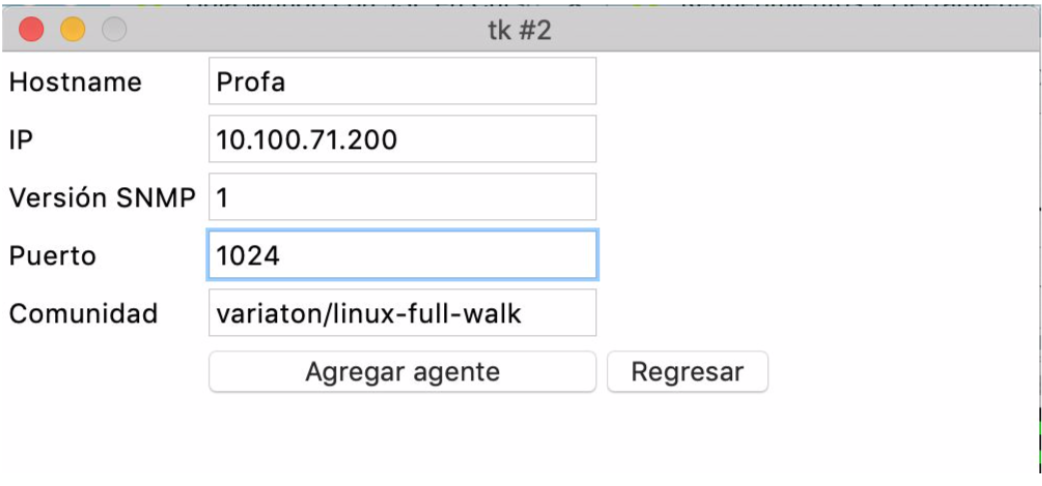
\includegraphics[scale=.8]{imagenes/primero/1-1.png}
    \caption{Agente}
\end{figure}
Una vez que fue ejecutado el programa y la lectura de los datos de uso de CPU se llevó a cabo en el plazo indicado, se obtuvo la siguiente tabla.
\begin{figure}[H]
  \centering
    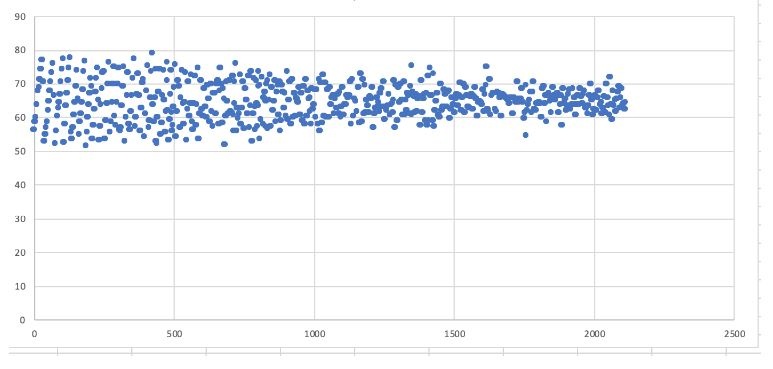
\includegraphics[scale=1]{imagenes/primero/1.JPG}
    \caption{Tabla de Dispersión}
\end{figure}
\subsection{Ejercicio 2: Mínimos Cuadrados}
\noindent
Una vez obtenidos los umbrales por medio de la tabla de dispersión se definieron dentro de nuestro sistema con el fin de poder hacer una predicción por medio del método de mínimos cuadrados, además en la gráfica se indica cuando ocurrirá un error y los colores varían cada que uno de los umbrales es rebasado; la línea de mejor ajuste se muestra de color amarillo.
\begin{figure}[H]
  \centering
    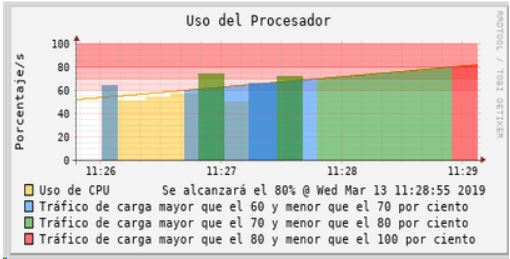
\includegraphics[scale=1.5]{imagenes/primero/2.JPG}
    \caption{Lectura del procesador}
\end{figure}
\noindent
En la gráfica se puede observar que el umbral GO es del 80\%. También, en las descripciones de la gráfica se encuentra el tiempo en el que el uso del CPU va a alcanzar ese umbral. Este tiempo es: 13 de marzo del 2019 a las 11:28:55. Para poder llevar a cabo este ejercicio se hizo uso del código siguiente.
\begin{figure}[H]
  \centering
    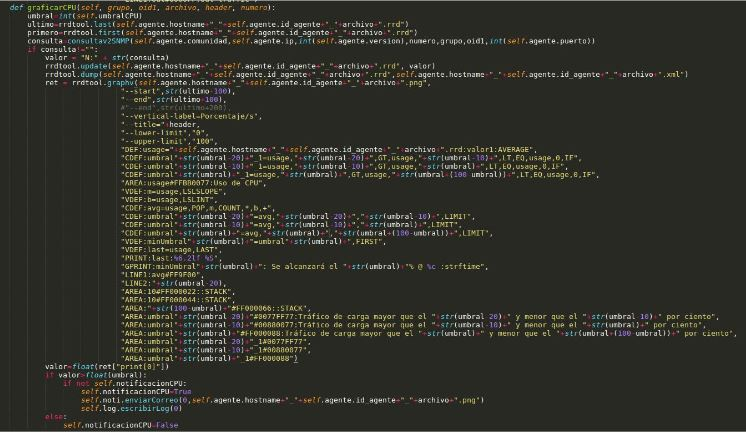
\includegraphics[scale=1]{imagenes/primero/3.JPG}
    \caption{Mínimos Cuadrados}
\end{figure}
\subsection{Ejercicio 3: Envío de Correos}
\noindent
Este ejercicio consistió en enviar un correo a la dirección de la profesora \textbf{tanibet.escom@gmail.com} en el momento en que se presentara una falla con fecha y hora del momento en el que ocurrió.
\begin{figure}[H]
  \centering
    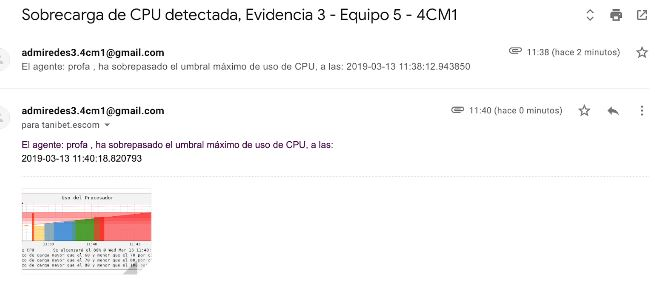
\includegraphics[scale=1.1]{imagenes/primero/4.JPG}
    \caption{Correo Enviado}
\end{figure}
\noindent
Para llevar a cabo este proceso se utilizó el siguiente código que nos permite crear el contenido de un correo y enviarlo a la dirección especificada con la información definida.
\begin{figure}[H]
  \centering
    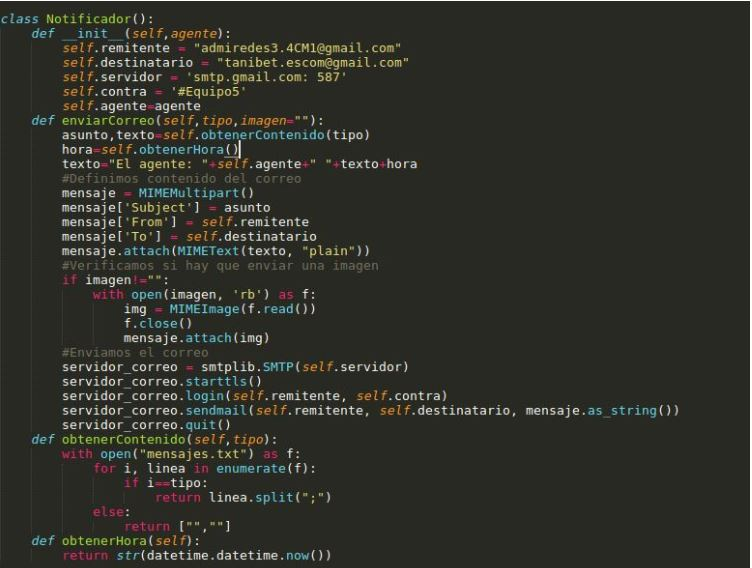
\includegraphics[scale=.8]{imagenes/primero/5.JPG}
    \caption{Envío de Correos}
\end{figure}
\subsection{Ejercicio 4: Lectura Completa}
\noindent
Para el ejercicio final, se tenia que llevar a cabo la lectura de los siguientes 3 parámetros: Uso de CPU, RAM y Disco Duro, además se tenían que mostrar las gráficas elaboradas en la práctica 1 y de igual manera, era necesario enviar el correo de notificación de que un error había ocurrido.
\begin{figure}[H]
  \centering
    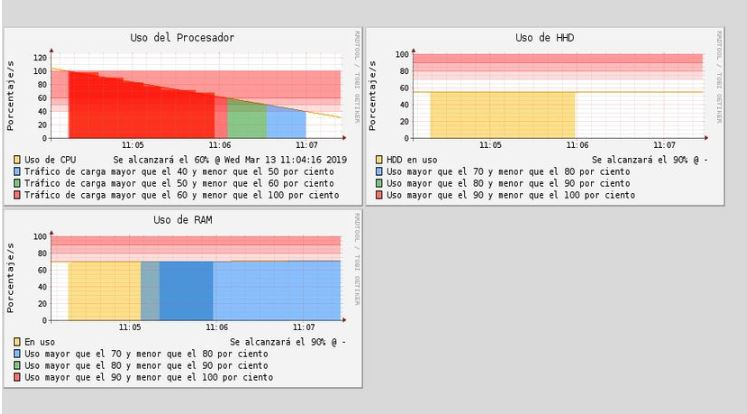
\includegraphics[scale=1]{imagenes/primero/6.JPG}
    \caption{Lectura de RAM,HDD y CPU}
\end{figure}
\begin{figure}[H]
  \centering
    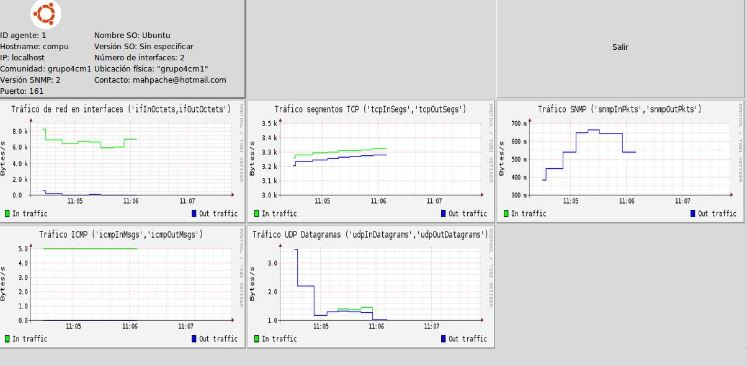
\includegraphics[scale=1]{imagenes/primero/7.JPG}
    \caption{Lectura de datos (Práctica 1)}
\end{figure}
\section{Examen 2.- Administración de fallas usando series de datos no lineales mediante Holt Winters}
\subsection{Evidencia 1}
Nos fue proporcionada una base de datos round robin (predict.rrd), el cual contenía las mediciones hechas para el objeto de la mib ``ifInOctets''. Esto con la finalidad de que nosotros determinaramos si los valores de alpha, beta y gamma eran los adecuado para realizar el monitoreo o podían mejorar.\\Para esto, lo primero que realizamos, fue graficar el archivo rrd con la intención de obtener información de esta gráfica. La gráfica obtenida puede observarse en la figura \ref{img:1-1}.
\begin{figure}[H]
  \centering
    
\includegraphics[scale=.75]{imagenes/segundo/1.png}
    \caption{Gráfica obtenida del archivo rrd}
    \label{img:1-1}
\end{figure}
Como se puede observar, la gráfica obtenida muestra el tráfico de entrada de color verde, los límites superior e inferior de color rojo y azul respectivamente, y la predicción de holt-winters de color rojo. Así como también el histórico de datos leidos de color gris.\\Posterior al análisis de la gráfica, se determino que los valores de alpha, beta y gamma se mantuvieran como los mismos, ya que la predicción era bastante cercana a los valores reales.\\Cabe señalar, que los valores de alpha, beta y gamma eran conocidos, gracias al ``dump'' hecho al archivo rdd, el cual genera un archivo xml desde el cual se pueden consultar estos valores.\\En caso de que hubiera sido necesario modificar el valor de alguno de estos valores, se puede usar la función ``tune'', con el cual se pueden modificar estos parámetros. Esto se puede observar en la figura \ref{img:1-2}.
\begin{figure}[H]
  \centering
    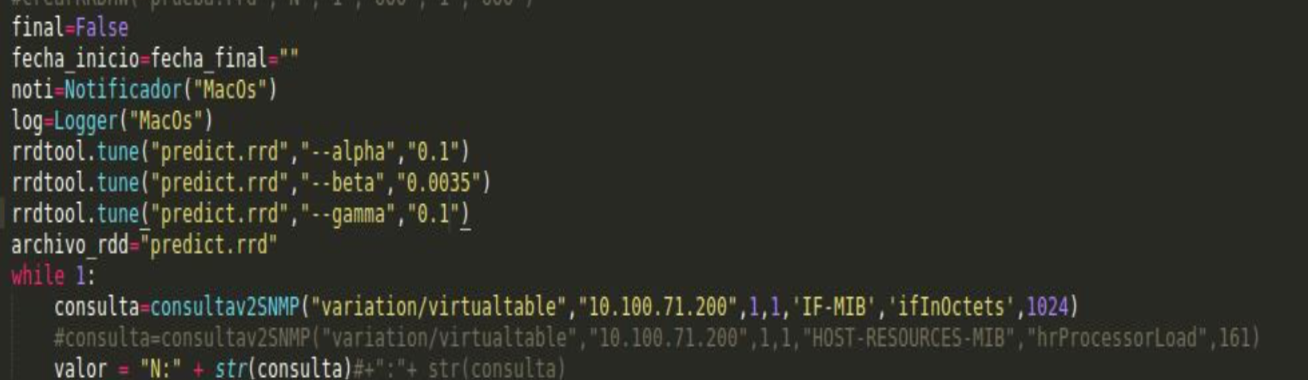
\includegraphics[scale=.75]{imagenes/segundo/2.png}
    \caption{Uso de la función tune}
    \label{img:1-2}
\end{figure}

\subsection{Evidencia 2}
Para la siguiente parte del examen, se nos pidió detectar una falla (comportamiento anormal que sobrepasas uno de los límites) y mostrar la gráfica correspondiente donde se observe como se coloea de color rojo el area donde se muestra la falla detectada.\\ En la figura \ref{img:1-3}
\begin{figure}[H]
  \centering
    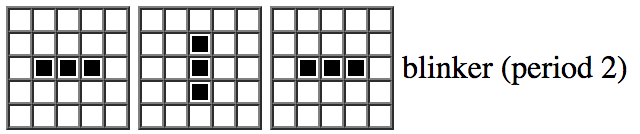
\includegraphics[scale=.75]{imagenes/segundo/3.png}
    \caption{Gráfica que muestra como se detecta un fallo}
    \label{img:1-3}
\end{figure}
Además, se nos solicito, que se mostrará el histórico de las mediciones hechas en un tiempo anterior al actual, esto puede observarse en la figura \ref{img:1-4} con el área marcada de color gris.
\begin{figure}[H]
  \centering
    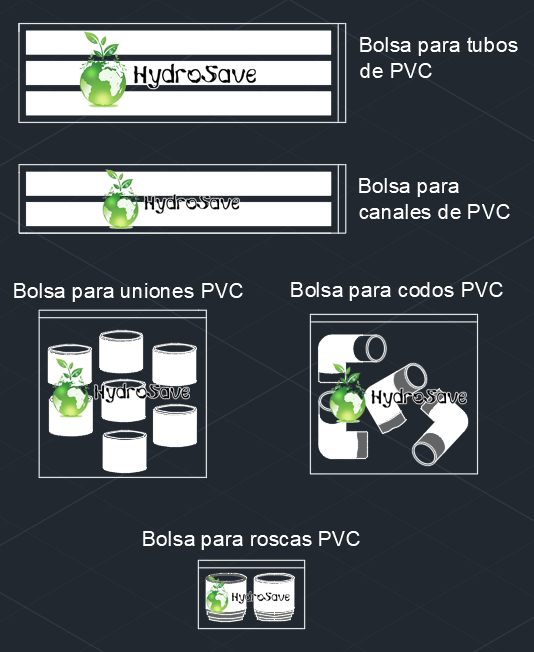
\includegraphics[scale=.75]{imagenes/segundo/4.png}
    \caption{Gráfica que muestra el histórico coloreado.}
    \label{img:1-4}
\end{figure}
\subsection{Evidencia 3}
Finalmente, fue necesario enviar una notificación al administrador, vía correo electrónico, cuando se presentarña alguna falla, estas notificaciones tenían que enviarse, al iniciar una falla y al culminar, en estas notificaciones, se incluye la información del agente donde se presentó el problema, la fecha y hora, y además una imagen que muestra la gráfica que es generada en tiempo real del rendimiento del objeto mib.\\En la figura \ref{img:1-5} se muestra uno de los correos que fue enviado.
\begin{figure}[H]
  \centering
    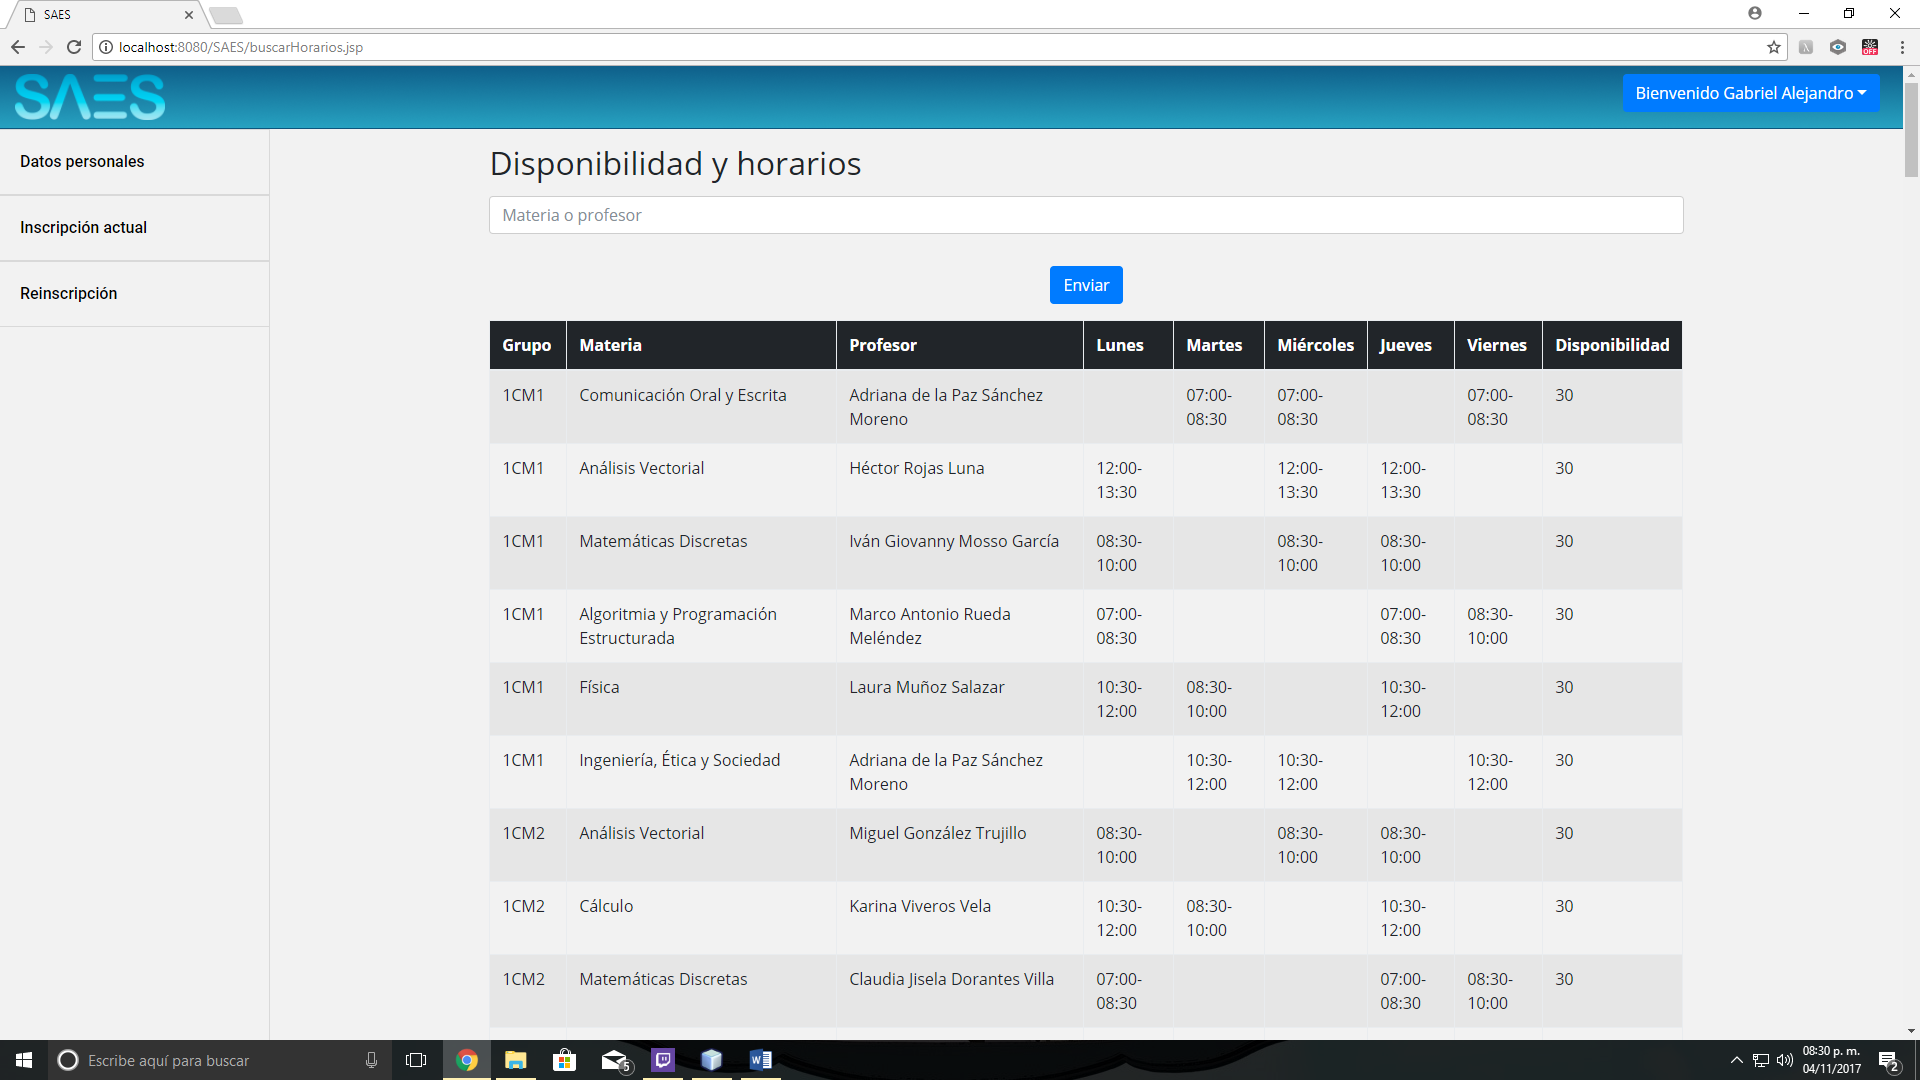
\includegraphics[scale=.75]{imagenes/segundo/5.png}
    \caption{Notificación enviada al detectarse una falla.}
    \label{img:1-5}
\end{figure}

\chapter{Códigos}
\section{Examen 1}
A continuación, se muestran los códigos elaborados para la realización del examen.

El archivo con el que se inicia la ejecución del programa, es con main.py, el cual solo crea una instancia del objeto Gestor, el cual se encuentra dentro del archivo gestor.py. Esto para ajustarnos al desarrollo orientado a objetos.\newline
main.py:
\lstinputlisting[language=Python]{src/primero/main.py}

El archivo gestor.py, es el que maneja toda la interfaz principal.\newline
gestor.py:
\lstinputlisting[language=Python]{src/primero/gestor.py}
Este archivo, maneja todo lo referente a los agentes.\newline
agente.py:
\lstinputlisting[language=Python]{src/primero/agente.py}
Este archivo, permite el registro de un nuevo agente.\newline
agregar\_agente.py:
\lstinputlisting[language=Python]{src/primero/agregaragente.py}
Ejemplo de como se almacena la información sobre los agentes, para la persistencia.\newline
agentes.json:
\lstinputlisting[language=Java]{src/primero/agentes.json}
Permite monitorear a un agente y además realiza la consultas correspondientes para mostrar las gráficas.\newline
monitor.py:
\lstinputlisting[language=Python]{src/primero/monitor.py}
Archivo en donde se encuentran todas las consultas necesarias para el correspondiente monitoreo.\newline
SNMP.py:
\lstinputlisting[language=Python]{src/primero/SNMP.py}
Posteriormente, para la detección de umbrales, se uso el siguiente código.\newline
detector\_umbrales.py:
\lstinputlisting[language=Python]{src/primero/detectorumbrales.py}
Para enviar los correos electrónicos de notificación cuando se sobrepasa un umbral se uso el código siguiente.\newline
notificador.py:
\lstinputlisting[language=Python]{src/primero/notificador.py}
Al igual que se envía una notificación, también se escribe en un archivo de log, el cual es controlado por el siguiente script.\newline
logger.py:
\lstinputlisting[language=Python]{src/primero/logger.py}

\section{Examen 2}
En este examen, se hizo uso de un script hecho en python el cual permite graficar un archivo rrd dado, el script usado es el siguiente.\newline
Graficador.py:
\lstinputlisting[language=Python]{src/segundo/Graficador.py}
Además se hizo uso del siguiente script que permite actualizar un archivo rrd con información nueva.\newline
P2Ejercicio5.py:
\lstinputlisting[language=Python]{src/segundo/P2Ejercicio5.py}
Y por último, se realizaron algunas modificaciones a los programas de notificación y logger que se mostraron en la sección anterior, el código se puede ver a continuación.\newline
notificador.py:
\lstinputlisting[language=Python]{src/segundo/notificador.py}
logger.py:
\lstinputlisting[language=Python]{src/segundo/logger.py}
\chapter{Conclusiones}
\noindent
\textbf{Hernández Pineda Miguel Angel:}\\
En el desarrollo de esta practica se trabajaron con dos algoritmos que nos permiten obtener la información cuando se presenta una falla, esto se puede traducir como el momento en que el comportamiento del objeto que se está monitorizando presenta un comportamiento anómalo, sin embargo la detección de dicho comportamiento varía de acuerdo con la lectura de los datos, pues si los datos recibidos tienen un comportamiento lineal se utilizan algunos algoritmos basados en predicción de datos mientras que los datos que tienen un comportamiento no lineal se utilizan algoritmos de muestreo y detección de errores.En esta ocasión los algoritmos utilizados fueron el de Mínimos cuadrados para el comportamiento lineal y Holt-Winters para el comportamiento no lineal. En cuestiones de implementación el algoritmo de Holt-Winters es más complicado debido a todos los parametros necesarios que deben definirse sobre la marcha para que el muestreo de la información sea satisfactorio y no se identifiquen errores donde no los hay por lo que, basados en su complejidad en la implementación, podemos decir que es bastante robusto y efectivo con los parámetros correctos.
\noindent
\\
\textbf{Monroy Martos Elioth:}\\
Considero que el desarrollo de esta práctica se fortalecieron distintas habilidades y hubo que hacer uso de varios conocimientos, sin embargo lo más importante desde mi perspectiva, es la importancia que hay detrás de un sistema de detección de fallas. Temas como mínimos cuadrados, métodos de linea base, método de Holt-Winters, e incluso una estrategia para la propuesta de umbrales para la detección de fallas, componen en conjunto una de las partes con mayor importancia funcional en nuestra herramienta. Además de que se desarrollaron varios scripts que resultan ser útiles para todo tipo de situaciones como el detector de umbrales programado, el logger, el notificador o el graficador. Los cuales pueden ser scripts que nos faciliten la vida en un futuro.\\
\noindent
\\
\textbf{Zuñiga Hernández Carlos:}\\
La práctica tuvo como principal objetivo la predicción del rendimiento y de fallas de los recursos disponibles en una computadora, así como la detección de fallas y el monitoreo del rendimiento en tiempo real. La predicción se implementó por medio de los algoritmos Mínimos cuadrados y Holt-Winters, cada uno con diferentes características; aunque Holt-winters demostró ser más preciso y eficiente, debido a que hacía uso de datos históricos para hacer la predicción. Es claro que es necesario monitorizar la actividad en los dispositivos que conforman una red, para que cuando se presente una falla, se pueda actuar a tiempo para resolverla o reducir el impacto y que todo el proceso que conlleva esta detección es complejo y debe hacerse de manera detallada.
%\newpage
\addcontentsline{toc}{chapter}{Referencias Bibliográficas}
\begin{thebibliography}{99}
\bibitem{IN1} CapItulo 20. Protocolo SSH. (n.d.). Retrieved May 19, 2019, from https://web.mit.edu/rhel-doc/4/RH-DOCS/rhel-rg-es-4/ch-ssh.html
\bibitem{IN1} HTTP. (n.d.). Retrieved May 19, 2019, from https://developer.mozilla.org/es/docs/Web/HTTPReferencias
\bibitem{IN1} Protocolo de transferencia de archivos. (2019, May 06). Retrieved May 19, 2019, from https://es.wikipedia.org/wiki/Protocolo-de-transferencia-de-archivos
\bibitem{IN1} ¿Qué es DNS? – Introducción a DNS - AWS. (n.d.). Retrieved May 19, 2019, from https://aws.amazon.com/es/route53/what-is-dns/
\bibitem{IN1} ¿Qué es un Servidor SMTP? Qué significa y cómo usarlo para enviar email. (2019, January 09). Retrieved May 19, 2019, from https://es.mailjet.com/blog/news/servidor-smtp/
\end{thebibliography}
\end{document}